\documentclass{sig-alternate-05-2015}
\usepackage[cache=false]{minted}
%\usepackage{caption}
\usepackage{hyperref}
\usepackage{amsmath}
\usepackage{listings}
%\newenvironment{code}{\captionsetup{type=listing}}{}
\usepackage{color}
\usepackage{url}

%\usepackage{inconsolata}


\definecolor{mygreen}{rgb}{0,0.6,0}
\definecolor{mygray}{rgb}{0.5,0.5,0.5}
\definecolor{mymauve}{rgb}{0.58,0,0.82}

\lstset{ %
	backgroundcolor=\color{white},   % choose the background color; you must add \usepackage{color} or \usepackage{xcolor}; should come as last argument
	basicstyle=\normalsize,        % the size of the fonts that are used for the code
	breakatwhitespace=true,         % sets if automatic breaks should only happen at whitespace
	breaklines=true,                 % sets automatic line breaking
	captionpos=b,                    % sets the caption-position to bottom
	commentstyle=\color{mygreen},    % comment style
	deletekeywords={...},            % if you want to delete keywords from the given language
	escapeinside={\%*}{*)},          % if you want to add LaTeX within your code
	extendedchars=true,              % lets you use non-ASCII characters; for 8-bits encodings only, does not work with UTF-8
	%frame=single,	                   % adds a frame around the code
	keepspaces=true,                 % keeps spaces in text, useful for keeping indentation of code (possibly needs columns=flexible)
	columns=fixed,
	keywordstyle=\bfseries\color{mygreen},       % keyword style
	language=C++,                 % the language of the code
	morekeywords={*,Nickel},           % if you want to add more keywords to the set
	%numbers=left,                    % where to put the line-numbers; possible values are (none, left, right)
	%numbersep=5pt,                   % how far the line-numbers are from the code
	%numberstyle=\tiny\color{mygray}, % the style that is used for the line-numbers
	%rulecolor=\color{black},         % if not set, the frame-color may be changed on line-breaks within not-black text (e.g. comments (green here))
	%showspaces=false,                % show spaces everywhere adding particular underscores; it overrides 'showstringspaces'
	%showstringspaces=false,          % underline spaces within strings only
	%showtabs=false,                  % show tabs within strings adding particular underscores
	%stepnumber=2,                    % the step between two line-numbers. If it's 1, each line will be numbered
	%stringstyle=\color{mymauve},     % string literal style
	tabsize=2	                   % sets default tabsize to 2 spaces
	%title=\lstname                   % show the filename of files included with \lstinputlisting; also try caption instead of title
}


\lstMakeShortInline[columns=fixed]|

\def\sharedaffiliation{%
\end{tabular}
\begin{tabular}{c}}

\begin{document}

\title{Tic-Tac-Tobot}
\subtitle{[EECS 149/249A Class Project]}

%\numberofauthors{2}
\author{
% 1st. author
%\alignauthor
Patrick Scheffe \\
\email{p.s@berkeley.edu} 
% 2nd. author
\and
Nikolas Alberti \\
\email{nikolas.alberti@berkeley.edu} 
% 3rd. author
\sharedaffiliation
\affaddr{Department of Electrical Engineering and Computer Science} \\
\affaddr{University of California}\\
\affaddr{Berkeley, CA} \\
}

\maketitle
\begin{abstract}

\end{abstract}

\section{Introduction}
Our charter defines the goal of this project as follows:

\emph{"In this project, we want to build a robot that will challenge you to play a game of tic-tac-toe. [...]The robot will control the movement of a whiteboard marker using two servos. The pen will be set up in a construction which has a shoulder and an elbow joint, so it can be moved to a defined x-y-position. The whiteboard is mounted in a fixed position next to the manipulator. First, the robot draws the playing field consisting of nine tiles. A camera will be used for monitoring the player's move (placing a circle or a cross). Autonomously, the robot will react and make its own move. In order to make space for the human player's moves, the whole construction should be able to move away from the field."}

This definition specifies well what the robot should be capable of doing. Accordingly, in order to meet the specification, a robotic manipulator must be assembled and controlled. Moreover, a computer vision component must be setup. At the end, everything must work together governed by a program that keeps track of the game and is able to compute own moves.
\section{Hardware}
\subsection{Arduino Uno}
The Arduino Uno is a microcontroller board equipped with an Atmel ATmega328P microcontroller \cite{Atm}. Arduino is an open-source hardware and software project originated in Ivrea, Italy\cite{Ard}. Hardware and software have been distributed by the founders of Arduino (known as Arduino LLC) and the producer of the official Arduino boards (Arduino S.r.l.). The goal of the Arduino project is to make the development on embedded systems as accessible as possible. For instance, the Arduino IDE, completely hides technical details like header files from the user.

The Arduino has 14 GPIO pins from which 6 support pulse width modulation (PWM). Because PWM is needed for controlling servo motors, that was the reason why we chose the Arduino as our platform along with the fact that the Arduino promised to offer an uncomplicated development.

\subsection{Servo Motors}
For the actuation, we used three Tower Pro MG90S servo motors\cite{Ser}. To connect them with the Arduino we used ordinary jumper cables. A 5V/2A power supply has been used in order to power the servo motors. Furthermore, a breadboard was used for distributing the power. Because the power supply originally ended in a coaxial power connector, we modified it have jumper cables as output for positive and negative voltage.

\subsection{Additional Materials}
Additionally, following materials have been used:
\begin{itemize}
	\item A Microsoft LifeCam HD-3000 webcam
	\item A white board
	\item Two white board markers
	\item Some screws, nuts and bolts
	\item ABS filament for 3D printing the custom parts
\end{itemize}

\section{Robotic Manipulator}
\subsection{Choosing the dimensions}
%TODO: citation Joo
For accurate two dimensional actuation, a classical robotic manipulator that  consists a chain of dependent joints is not suitable for a low budget approach. The plotclock, a project by Johannes ``\emph{Joo}'' Heberlein from the Fablab Nuremberg (comparable to a makerspace) impressively proved a way to make low budget 2D actuation work \cite{Joo}. Therefore, we planed to chose a similar manipulator. However, while the plotclock needs to cover a range whose dimensions in x-direction exceed the dimensions in y-direction, it was not possible to blindly adapt the manipulator. For our project, actuation needs to be performed in an area formed like a square. Therefore, we needed to resize the limbs.

This problem can be described as a maximization problem:
 The desired area of the largest possible square that fits into the reachable range of the actuator is given. Find the dimensions $L_1$, $L_2$ and $L_3$ that minimize the sum $L_1 + L_2 +L_3$.
 
 Unfortunately, the function of the largest reachable square $A(L_1, L_2, L_3)$ is not defined by a function that allows for partly deriving towards $L_1$, $L_2$ and $L_3$ and setting the derivations to zero. 
 We therefore chose to model the reachable space in a geometry software called \emph{Geogebra}, an open source software for supporting mathematical education in schools and universities\cite{Geo}. Then, we empirically derived a near optimal sizing that yields a reachable square of approximately $100 cm^2$(\autoref{fig:sketch}). A constraint was that we wanted the player to face the robot like they would sit on opposite ends of a table. Consequently, choosing orientation of the square freely to allow a better usage of the space was not possible.

 \begin{figure}
 	\centering
 	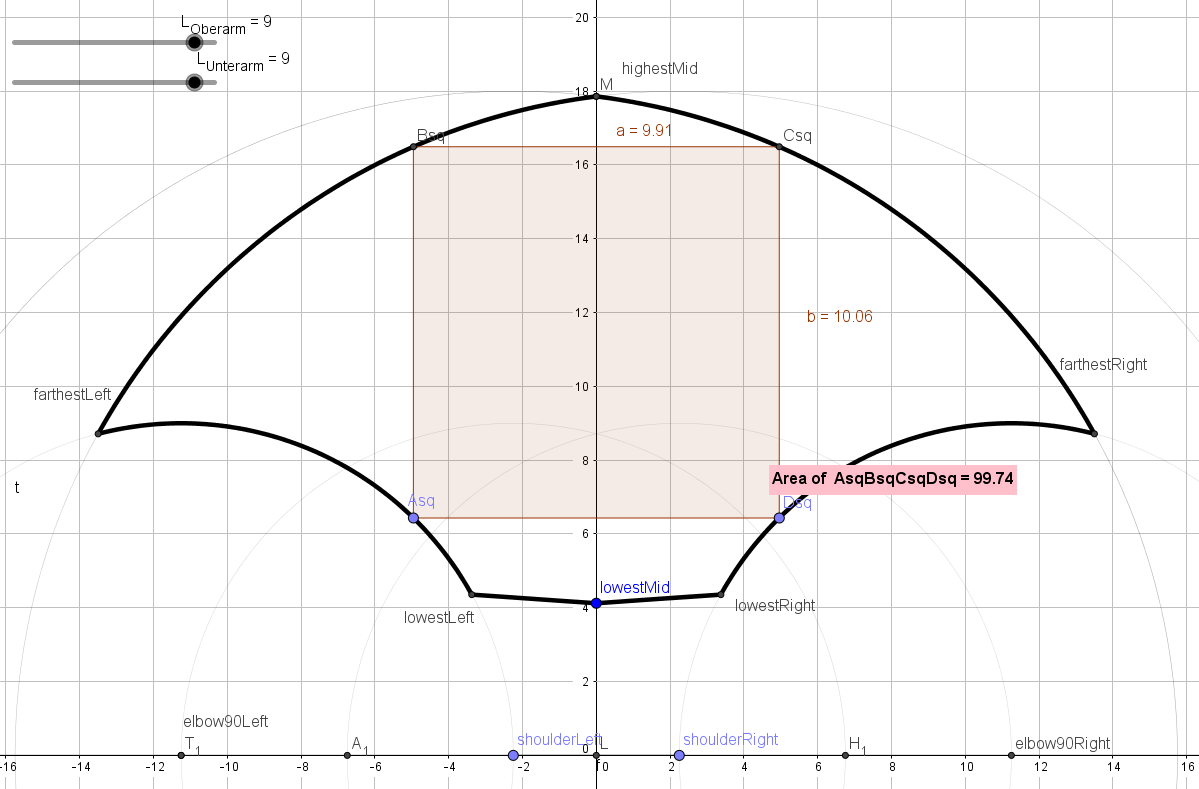
\includegraphics[width=.42\textwidth]{img/sizing.png}
    \caption{Geogebra Sketch Used for Sizing}
 \end{figure}
\subsection{Manufacturing}
\subsection{Simplified Kinematic Model}\label{section1}

A simplified sketch of the robotic manipulator can be seen in  \autoref{fig:model}.
As a first approximation it is useful to determine the angles $\theta_1$ to $\theta_4$ from the given position of the joint at which the two arms coincide (x,y). The key for solving this inverse kinematics problem is to divide it into smaller subproblems that each can be solved individually. For that purpose, the line segments $a$, $b$ and $c$ are introduced.
\begin{figure}[!h]
	\centering
	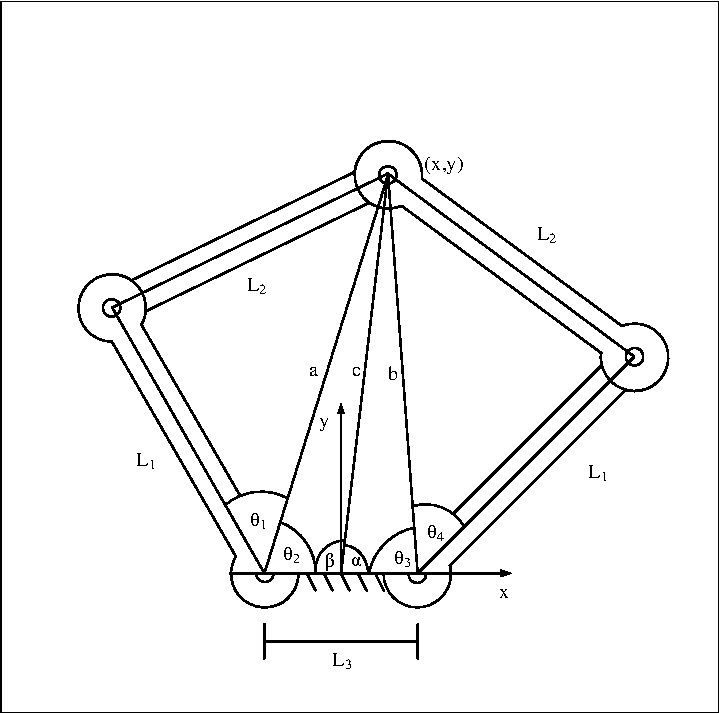
\includegraphics[width=.42\textwidth]{img/LinkDiagramSimple_try.pdf}
	\caption{Simplified Version of the Manipulator}\label{fig:model}\label{fig:sketch}
\end{figure}

From the initial information, following values can be directly computed:
\begin{align*}
\alpha &= \arctan \left( \frac{y}{x} \right) \\
\beta  &= \pi - \alpha \\
c      &= \sqrt{x^2 + y^2}\\
a      &= \sqrt{\left(x+ \frac{L_3}{2}\right)^2 + y^2}\\
b      &=\sqrt{\left(x- \frac{L_3}{2}\right)^2 + y^2}
\end{align*}


Now, you can solve for $\theta_2$ and $\theta_3$ by either using sine rule or cosine rule. However, the sine rule can be ambiguous in certain setups, which makes case differentiation necessary. Although mathematically steady, in our implementation the domain crossing from one solution to the other resulted in discontinuities of the movement. Therefore, the unambiguous cosine rule solution is preferred:
\begin{align*}
\theta_2 &= arccos\left(  \frac{a^2 + (\frac{L_3}{2})^2 - c^2}{aL_3} \right)\\
\theta_3 &= arccos\left(  \frac{b^2 + (\frac{L_3}{2})^2 - c^2}{bL_3} \right)\\
\intertext{Using cosine rule we can also solve for $\theta_1$ and $\theta_4$:}
\theta_1 &= arccos\left(  \frac{a^2 + {L_1}^2 - {L_2}^2}{2aL_1} \right)\\
\theta_4 &= arccos\left(  \frac{b^2 + {L_1}^2 - {L_2}^2}{2bL_1} \right)
\end{align*}

\subsection{Complete Kinematic Model}
The simplified version of the kinematic model is good for quickly creating a working implementation. However, any movements executed by the manipulator will suffer from distortion. The pen is not mounted \emph{exactly} at the joint's position but in a small distance. Hence, a precise solution is necessary. For that purpose, new definitions must be made (\autoref{fig:model2}).
\begin{figure}[!h]
	\centering
	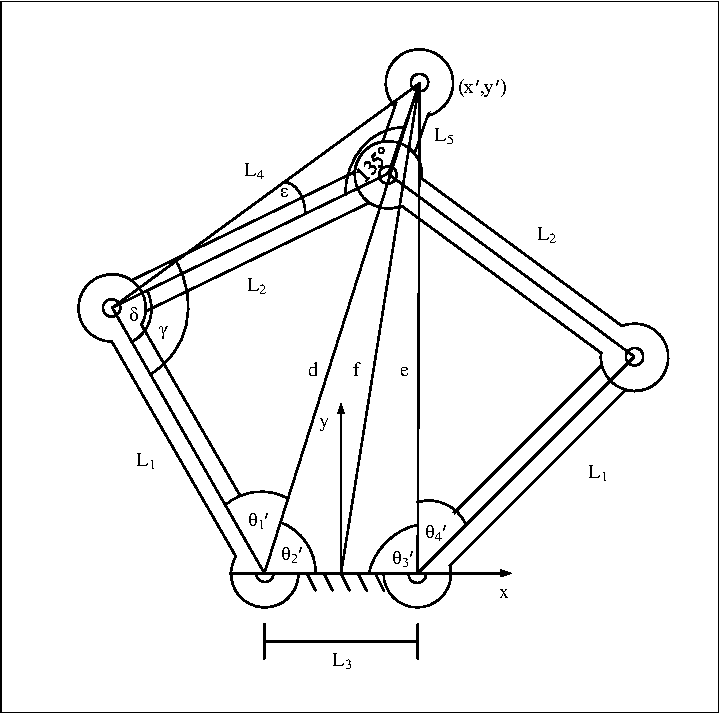
\includegraphics[width=.42\textwidth]{img/LinkDiagramComplicated_try.pdf}
	\caption{Complete Version of the Manipulator}\label{fig:model2}
\end{figure}

$L_4$ and $\epsilon$ are fixed measures and not influenced by the position of the manipulator:
\begin{align*}
L_4 &= \sqrt{{L_2}^2 + {L_5}^2 - 2L_5L_2cos\left(\frac{3\pi}{4}\right)}\\
\epsilon &= arccos\left(  \frac{{L_4}^2 + {L_2}^2 - {L_5}^2}{2L_4L_2} \right)\end{align*}
$d$, $e$ and $f$ can be yielded by the Pythagorean theorem:
\begin{align*}
f &= \sqrt{{x'}^2 + {y'}^2}\\
d &= \sqrt{\left(x'+ \frac{L_3}{2}\right)^2 + {y'}^2}\\
e &= \sqrt{\left(x'- \frac{L_3}{2}\right)^2 + {y'}^2}
\end{align*}
Now, $\theta_2'$, $\theta_3'$ and $\delta$ can be computed using cosine rule:
\begin{align*}
\theta_2' &= arccos\left(  \frac{d^2 + (\frac{L_3}{2})^2 - f^2}{dL_3} \right)\\
\theta_3' &= arccos\left(  \frac{e^2 + (\frac{L_3}{2})^2 - f^2}{eL_3} \right)\\
\delta    &= arccos\left(  \frac{{L_4}^2 + {L_1}^2 - d^2}{2L_4L_1} \right)
\end{align*}
$\delta$ is the sum of $\epsilon$ and $\gamma$.
\begin{align*}
\gamma &= \delta - \epsilon
\end{align*}
That allows us to calculate some quantities of the simple kinematics model:
\begin{align*}
a 		 &= \sqrt{{L_1}^2 + {L_1}^2 - 2L_1L_2cos\left(\gamma\right)}\\
\theta_1 &= arccos\left(  \frac{a^2 + {L_1}^2 - {L_2}^2}{2aL_1} \right)\\
\theta_2 &= \theta_1' + \theta_2' - \theta_1
\end{align*}
Finally, we are able to find the position of the joint at which the two arms coincide:
\begin{align*}
y &= a \sin(\theta_2)\\
x &= a\cos(\theta_2) - \frac{L_3}{2}
\end{align*}

Now, the methods from \autoref{section1} can be used to solve for $\theta_3$ and $\theta_4$.
\subsection{Modeling the Servo Motors}
Servo motors are motors that do not support continuous motion but in return precisely can be driven to a desired angle. They have three external cables in different colors. The black cable should be connected to ground and the red one to $V_{DD}$ (roughly 5V). These two cables supply the servo motor with the necessary power. The third cable (white, yellow or orange) carries the control signal. The control is done by PWM. The servo motor expects to receive a pulse every 20\,ms with a pulse width between 1\,ms and 2\,ms. By proportional control, the servo motor assumes its most positive position at the the pulse width of 1\,ms and the most negative position at a pulse width of 2\,ms as defined in the mathematical direction of rotation. The range in between these extrema can be assumed to be linearly covered, i.e. a pulse width of 1.5\,ms should yield the position in between these positions. A function can be derived that maps the pulse width to an angular position of the servomotor:
\begin{align*}
	\text{Angle}(t_\text{pulse}) =~& \frac{t_\text{pulse} -1\,\text{ms} }{2\,\text{ms}-1\,\text{ms}}\cdot \left(\text{Angle}_{max}-\text{Angle}_{min}\right) \\ & + \text{Angle}_{min}, \qquad 1\,\text{ms} \le t_\text{pulse}\le 2\,\text{ms}
\end{align*}

%\begin{eqnarray}
%Angle(t_{pulse}) &=& \frac{t_{pulse} -1 \text{ms} }{2 \text{ms}-1 \text{ms}}\cdot \left(Angle_{max}-Angle_{min}\right)&\nonumber \\ &&+Angle_{min},&1 \text{ms} \le t_{pulse}\le 2 \text{ms}  \nonumber
%\end{eqnarray}
This is just a model of the movement of the servo motors. There are three causes that the actual behavior deviates from the model:
\begin{itemize}
	\item A high torque forces the servo motors from leaving its desired position.
	\item The backlash of the gears in the servo motors adds an inaccuracy to the position.
	\item Non-linearities make the servomotor cover the range of movement not evenly.
\end{itemize}
Furthermore, when the pulse width modulation signal is created by a digital signal, a quantization error occurs.
As you can see, the model is making some approximations. The inner of the servo motor is treated as black box. However, adding the details would bloat the model and the gain is questionable. The proposed model is precise enough to be useful but not so complex that it becomes cumbersome.

\section{Software on the Arduino}
\subsection{Overview over the software structure}
Every program written with the Arduino IDE consists of the function |void init()| and |void loop()|. The |init()| function is executed once at startup and afterwards the Arduino keeps looping through the |loop()| function. That is, because as a typical microcontroller, the Atmel ATmega328P, does not have an operating system and can not just end a task. In addition, following major functions have been defined:

\begin{itemize}
	\item |void lower()| lowers the marker.
	\item |void lift()| removes the marker from the surface.
	\item |void calculateServoMap(double x_prime,|\\|double y_prime,double* servoLsoll,|\\|double* servoRsoll)|
	 calculates the values that should be written to the servo motors given an x-y-position.
	\item |void set_servos(double x, double y)| calls\\ |calculateServoMap| and writes to the servo motors.
	\item  |void go_to (double xto, double yto)| interpolates between the current position and the desired position of the manipulator and successively sets the position of the servo motors using |set_servos()| in order to achieve a smooth movement between the origin and the destination position.
	\item |void draw_{cross,circle}(double x_offset, double y_offset)| draws cross/circle to any position defined by a passed x-y-position.
	\item |draw_field()| draws the playing field.
\end{itemize}

The main functionality is implemented in the |loop()| function: The processor waits for an instruction coded in a byte send from the master. Once it receives the command, it is executed and following an acknowledgment is sent that it has finished the execution.

\subsection{Controlling the Servo Motors}
The Arduino Uno has six PWM pins available.
Very conveniently, the Arduino IDE already is equipped with a library |Servo|. This library allows us to instantiate objects of the type |Servo|. The most important functions on this object are |attach()| and |write()|. The |attach()| function assigns the Servo object to a GPIO pin. The |write()| maps an angle in the range of $0^\circ$ to $180^\circ$ to a pulse width and makes the attached GPIO pin assume the according PWM. Inherently, a reachable range of $180^\circ$ is assumed for the servo motor. However, our servo motors only are capable of spinning $150^\circ$. Signals that exceed the range of approximately $15^\circ$ to $165^\circ$ simply have been ignored.

Additionally,the gear that is on top of the servo motor did not allow us to attach the hat that enables us to move the limbs in any desired way. Therefore, the angle due to this offset also needed to be considered. 
%\begin{code}
%	\captionof{listing}{Angle Conversion}
%\begin{minted}{c++}
\begin{lstlisting}[caption = Finding the right angle]
#define leftMax 161
#define rightMax 16
...
void calculateServoMap(...){
...
*servoLsoll = leftMax - (pi - (theta1+theta2) ) * 180/pi; 
*servoRsoll = rightMax + (pi - (theta3+theta4) ) * 180/pi;
}
\end{lstlisting}
%\end{minted}
%\end{Code}

\section{Software on the Computer}
\subsection{Computer Vision}
\subsection{Tic-Tac-Toe AI}
As a simple and well known game, tic-tac-toe already is fully explored and algorithms to optimally play the game are available. Also, the relatively state space of the board make exhaustive search for an optimal solution possible. The concept of the algorithm used in our implementation is nicely explained in \cite{NSB}.
Furthermore, \cite{vdS} provides a similar implementation of the game in Python. Although it heavily relies on the functions only available in a GUI environment, it served as a useful reference.

Since the detailed explanation can be read in \cite{NSB}, the principle here should only summarized: A $3\times 3$ 2D-array of represents the nine gaps in the field. On each move, the algorithm iterates over the gaps and when it encounters an empty gap, it recursively calls itself. Doing so, an altered board with the new move and another active player is passed. The break condition is either that one of the players has won or there is no free gap anymore. The original caller chooses the move that has offers the best outcome with in case of a win minimum and in case of a defeat maximum number of recursive calls. It is a typical example of a minimax algorithm.

The described algorithm plays optimally, in a meaning that it is impossible to win against it. Also, in case a win can be enforced, the computer finds this optimal path to the win. Still, it lacks an understanding for common human mistakes and assumes the opponent to play optimally himself.

In order to offer some kind of a sense of achievement to the player with a probability of 15\% the algorithm is disabled and a random move is made.
\subsection{The Game Program}
Having described each part separately, the only thing left is combining each part to form the robot that autonomously plays Tic-Tac-Toe. A superordinate loop sets up the playing field and makes the player decide whether he wants to start or not. In order to completely decouple the game from input at the computer, we made the design choice that the first player's sign is the cross and the second player's sign is the circle. With that definition, the dialog whether the player or the computer should start the game completely can be done by drawing either a cross (``I want to start!'') or a circle (``The computer should start!'') to the right of the playing field.

Once the setup is done, a subordinate loop is started that breaks after nine subsequent moves or when on one of the players has won.

For the serial communication with the Arduino, the library |pyserial| \cite{PyS} has been used.

\bibliographystyle{plain}
%\bibliography{sigproc}

\begin{thebibliography}{Atm}
	
	\bibitem[Atm]{Atm}
	Atmel: \emph{\href{https://cdn.sparkfun.com/datasheets/Kits/doc8161.pdf.}{ATmega328P Manual}}
	
	\bibitem[Ard]{Ard}
	{Arduino LLC:
	\emph{\href{https://www.arduino.cc/en/Main/ArduinoBoardUno}{Arduino UNO \& Genuino UNO}}}
	
	\bibitem[Ser]{Ser}
	Adafruit: \emph{\href{https://www.adafruit.com/products/1143}{Micro Servo - MG90S High Torque Metal Gear}}
	
	\bibitem[Joo]{Joo}
	Johannes ``Joo'' Heberlein: \emph{\href{http://www.thingiverse.com/thing:248009}{Plotclock}}, Nuremberg(2014), published under the \href{https://creativecommons.org/licenses/by/3.0/}{Creative Commons - Attribution license}
	
	\bibitem[Geo]{Geo}
	Markus Hohenwarter et al.: \emph{\href{geogebra.org}{Geogebra}}, software published under a \href{https://www.geogebra.org/license}{free, non-commercial license}; \href{https://dev.geogebra.org/trac}{source code} published under the \href{http://www.gnu.org/licenses/gpl.html}{GNU General Public License}
	
	\bibitem[NSB]{NSB}
	{Never Stop Building LLC}: \emph{\href{http://neverstopbuilding.com/minimax}{Tic Tac Toe: Under standing The Minimax Algorithm}(2013)}
	
	\bibitem[vdS]{vdS}
	Mauritz van der Schee: \emph{\href{https://www.leaseweb.com/labs/2013/12/python-tictactoe-tk-minimax-ai/}{Python TicTacToe with Tk and minimax AI}}(2013)
	
	\bibitem[PyS]{PyS}
	Chris Liechti:\href{https://pythonhosted.org/pyserial/}{pyserial}(2001)
	
\end{thebibliography}

\end{document}